\section{Presentation Markup}

\subsection{Introduction}

\subsubsection{Box Model}

User agents must also follow the rules described in section 4.7.14
Embedded content, MathML of \cite{HTML5}, in particular the equivalence with
implicit {\tt mtext} and {\tt merror} to handle non-conforming MathML markup.

MathML elements have the following box model. The {\tt <math>} root may have
inline or block display while tabular MathML elements have table, table-row and
table-cell display (see ????). The {\tt <math>} and {\tt <mtd>} elements
generate an anonymous {\tt <mrow>} MathML box child that contains the boxes of
their children and use the box parameters below to layout this anonymous
{\tt <mrow>} box.
No line breaking can happen within MathML boxes and the min-content width is
equal to the max-content width, these are simply called the intrinsic width.
Each MathML box has the following parameters:

\begin{enumerate}
\item intrinsic width $W$.
\item logical width $w$, ascent above the origin $a$ and descent below the
  origin $b$. The height is then $a+b$.
\item ink ascent $A$ and descent $B$, corresponding to the exact box enclosing
  ink of text and bars within the MathML box.
\end{enumerate}

\begin{figure}
\centering
\begin{tikzpicture}[yscale=-1]
  \draw[->] (0,0) -- (15,0) node[below] {$x$};
  \draw[->] (0,0) -- (0,6) node[right] {$y$};
  \draw[dashed,blue] (0,-2) -- (13.5,-2) -- (13.5,4) -- (0,4) -- cycle;
  \MathMLBox{0}{0}{1}{1}{red}
  \MathMLBoxMetrics{0}{0}{1}{1}{red}{1}
  \MathMLBox{6}{2}{1.5}{1}{green}
  \MathMLBoxMetrics{6}{2}{1.5}{1}{green}{2}
\end{tikzpicture}
\label{MathMLBoxModel}
\end{figure}

For MathML element containing only text nodes or foreign elements, we assume
that the content is simple enough to determine these values. For example,
in most case, this is just a single text node and $w = W$.
A MathML element containing only other MathML elements follow special rules to
layout their children at position $(x_i,y_i)$ with parameters
$W_i,w_i,a_i,b_i,A_i,B_i$. Then as a general rule, its box parameters are given
by taking the union of child boxes, that is:
%
$$w = \left(\max_{1 \leq i \leq n } {x_i + w_i}\right) -
      \left(\min_{1 \leq i \leq n} x_i\right)$$
$$W = \left(\max_{1 \leq i \leq n } {x_i + W_i}\right) -
      \left(\min_{1 \leq i \leq n} x_i\right)$$
$$a = \max_{1 \leq i \leq n } {a_i - y_i}$$
$$b = \max_{1 \leq i \leq n } {b_i + y_i}$$
$$A = \max_{1 \leq i \leq n } {A_i - y_i}$$
$$B = \max_{1 \leq i \leq n } {B_i + y_i}$$
%

Note that the schemas in this specification are drawn assuming left-to-right
directionality. If the CSS {\tt direction} is set to right-to-left, then the
elements should be layout by making the $x$-axis pointing from right-to-left.

Detailed rules as well as possible additional spacing are given in ????

\subsection{Token Elements}

...

\subsection{General Layout Schemata}

\subsubsection{Horizontally Group Sub-Expressions {\tt <mrow>}}

...

\subsubsection{Fractions {\tt <mfrac>}}

The MathML specification describes {\tt mfrac} as follows \cite{MathML3}:
%
\begin{quote}
The {\tt mfrac} element is used for fractions. It can also be used to mark up
fraction-like objects such as binomial coefficients and Legendre symbols.
The syntax for {\tt mfrac} is
%
\begin{lstlisting}
  <mfrac> numerator denominator </mfrac>
\end{lstlisting}
%
The {\tt mfrac} element sets {\tt displaystyle} to "false", or if it was
already false increments {\tt scriptlevel} by 1, within numerator and
denominator.
\end{quote}

The {\tt displaystyle} and {\tt scriptlevel} changes be achieved with the
following style in the user agent stylesheet (section \ref{UAStylesheet}):
%
\begin{lstlisting}
  mfrac > * {
    mathml-script-level: auto;
    mathml-math-style: inline;
  }
\end{lstlisting}
%
The default line thickness is given by {\tt FractionRuleThickness}
Use the {\tt linethickness} attribute \cite{MathML3} to determine the
actual thickness of the fraction bar. A percent or unitless length is
interpreted as a multiple of the default rule thickness and
the named values "thin", "medium" and "thick" are interpreted as
50\%, 100\%, 200\%.
The color and visibility of the fraction bar must honor the values given by the
{\tt color} and {\tt visibility} CSS properties on the {\tt mfrac} element.

If the actual line thickness is nonzero, the {\tt mfrac} element is laid out as
shown on figure \ref{FractionBoxModel}.
The width is given by the maximum width of the
numerator and denominator and the numerator and denominator are horizontally
centered. A fraction bar with the actual thickness is drawn centered on the
axis height. The numerator and denominator are shifted
up and down using the values {\tt FractionNumeratorShiftUp},
{\tt FractionDenominatorShiftDown} in inline style and
{\tt FractionNumeratorDisplayStyleShiftUp},
{\tt FractionDenominatorDisplayStyleShiftDown} in display style.
If necessary, these shift values are increased to ensure that the gaps between
the numerator/denominator and fraction bar satisfy the minimal values provided
by {\tt FractionDenominatorGapMin} and
{\tt FractionNumeratorGapMin} in inline style and
{\tt FractionDenominatorDisplayStyleGapMin} and
{\tt FractionNumeratorDisplayStyleGapMin} in display style.

\begin{figure}
\centering
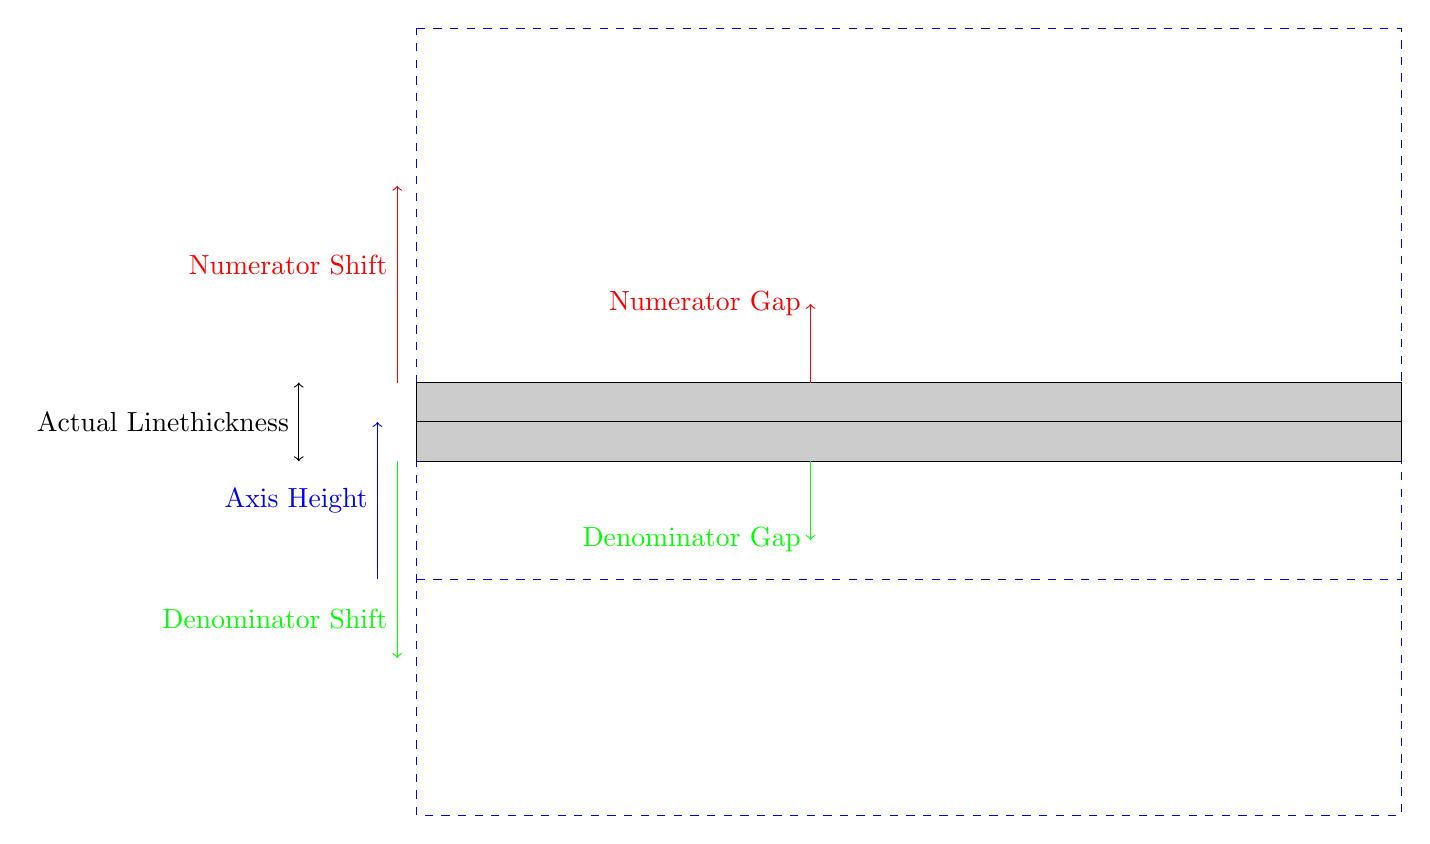
\begin{tikzpicture}[yscale=-1]
  \MathMLBox{0}{-5}{2.5}{1}{red}
  \MathMLBox{3.75}{1}{1}{1}{green}
  \draw[dashed,blue] (0,-7) -- (12.5,-7) -- (12.5,3) -- (0,3) -- cycle
  (0,0) -- (12.5,0);
  \fill[black!20] (0,-2.5) -- (12.5,-2.5) -- (12.5,-1.5) -- (0,-1.5) -- cycle;
  \draw[black] (0,-2.5) -- (12.5,-2.5) -- (12.5,-1.5) -- (0,-1.5) -- cycle
  (0,-2) -- (12.5,-2);
  \draw[->,blue] (-.5,0) -- (-.5,-1) node[left]{Axis Height} -- (-.5,-2);
  \draw[<->,black] (-1.5,-2.5) --
  (-1.5,-2) node[left]{Actual Linethickness} -- (-1.5,-1.5);
  \draw[->,red] (-.25,-2.5) -- (-.25,-4)
  node[left]{Numerator Shift} -- (-.25,-5);
  \draw[->,green] (-.25,-1.5) -- (-.25,.5)
  node[left]{Denominator Shift} -- (-.25,1);
  \draw[->,red] (5,-2.5) -- (5,-3.5) node[left]{Numerator Gap};
  \draw[->,green] (5,-1.5) -- (5,-.5) node[left]{Denominator Gap};
\end{tikzpicture}
\label{FractionBoxModel}
\end{figure}

If the actual line thickness is zero,
the {\tt mfrac} element is instead laid out as
shown on figure \ref{StackBoxModel}. The gap between the top and bottom boxes
is equally split around the axis height. The relevant shift values are now
{\tt StackTopShiftUp},
{\tt StackBottomShiftDown} in inline style and
{\tt StackTopDisplayStyleShiftUp},
{\tt StackBottomDisplayStyleShiftDown} in display style.
If necessary, the two shift values are increased by a same value to ensure
the gap between the top and bottom boxes satisfy the values provided by
by {\tt StackGapMin} in inline style and
{\tt StackDisplayStyleGapMin} in display style.

\begin{figure}
\centering
\begin{tikzpicture}[yscale=-1]
  \MathMLBox{0}{-5}{2.5}{1}{red}
  \MathMLBox{3.75}{1}{1}{1}{green}
  \draw[dashed,blue] (0,-7) -- (12.5,-7) -- (12.5,3) -- (0,3) -- cycle
  (0,0) -- (12.5,0);
  \draw[black,dashed] (0,-2) -- (12.5,-2);
  \draw[->,blue] (-.5,0) -- (-.5,-1) node[left]{Axis Height} -- (-.5,-2);
  \draw[->,red] (-.25,-2) -- (-.25,-4)
  node[left]{Stack Top Shift} -- (-.25,-5);
  \draw[->,green] (-.25,-2) -- (-.25,.5)
  node[left]{Stack Bottom Shift} -- (-.25,1);
  \draw[<->,blue] (5,-3.5) -- (5,-1.5) node[left]{Stack Gap} --
  (5,-.5);
\end{tikzpicture}
\label{StackBoxModel}
\end{figure}

If the numerator is an embellished operator and the {\tt mfrac} element is the
outermost element in this embellished operator hierarchy then the operator
leading and trailing spaces must be added around the fraction.
(TODO: Gecko always adds 1px around the fraction)

User agents may extend the box model to support the {\tt numalign},
{\tt denomalign} and {\tt bevelled} attributes \cite{MathML3}.

\subsubsection{Radicals {\tt <msqrt>}, {\tt <mroot>}}

The MathML specification describes radicals as follows \cite{MathML3}:
%
\begin{quote}
These elements construct radicals. The {\tt msqrt} element is used for square
roots, while the {\tt mroot} element is used to draw radicals with indices,
e.g. a cube root. The syntax for these elements is:
%
\begin{lstlisting}
  <msqrt> base </msqrt>
  <mroot> base index </mroot>
\end{lstlisting}
%
The {\tt mroot} element requires exactly 2 arguments. However, {\tt msqrt}
accepts a single argument, possibly being an inferred {\tt mrow} of multiple
children.

The {\tt mroot} element increments scriptlevel by 2, and sets displaystyle to
"false", within index, but leaves both attributes unchanged within base. The
{\tt msqrt} element leaves both attributes unchanged within its argument. [...]

Note that in a RTL directionality, the surd begins on the right, rather than
the left, along with the index in the case of mroot.
\end{quote}

The {\tt displaystyle} and {\tt scriptlevel} changes be achieved with the
following style in the user agent stylesheet (section \ref{UAStylesheet}):
%
\begin{lstlisting}
  mroot > :not(:first-child) {
    mathml-script-level: +2;
    mathml-math-style: inline;
  }
\end{lstlisting}

The line thickness of the overbar is given by {\tt RadicalRuleThickness}.
The gap between the overbar and base is given by {\tt RadicalVerticalGap}
in inline style and {\tt RadicalDisplayStyleVerticalGap} in display style.
The ascent above the overbase is given by {\tt RadicalExtraAscender}. The
surd is drawn by trying to vertically stretch the character U+221A SQUARE ROOT
to at least the sum of the ink height of the base, the radical gap and the
radical rule thickness. If the CSS {\tt direction} is set to right-to-left,
then the surd is actually drawn from the glyph obtained by mirroring
U+221A SQUARE ROOT via the {\tt rtlm} OpenType feature.
The color and visibility of the surd and overbar must honor the values given by
the {\tt color} and {\tt visibility} CSS properties on the {\tt msqrt} element.

The {\tt msqrt} element is laid out as shown on figure \ref{SquareRootBoxModel}.
The width is given by the sum of the width of the surd and of the base.
The baseline of the square root matches the baseline of the base.
The ink box is determined from the ink boxes of the surd and base while the
logical box takes into account the extra ascender
(add an extra descender ?????).

\begin{figure}
\centering
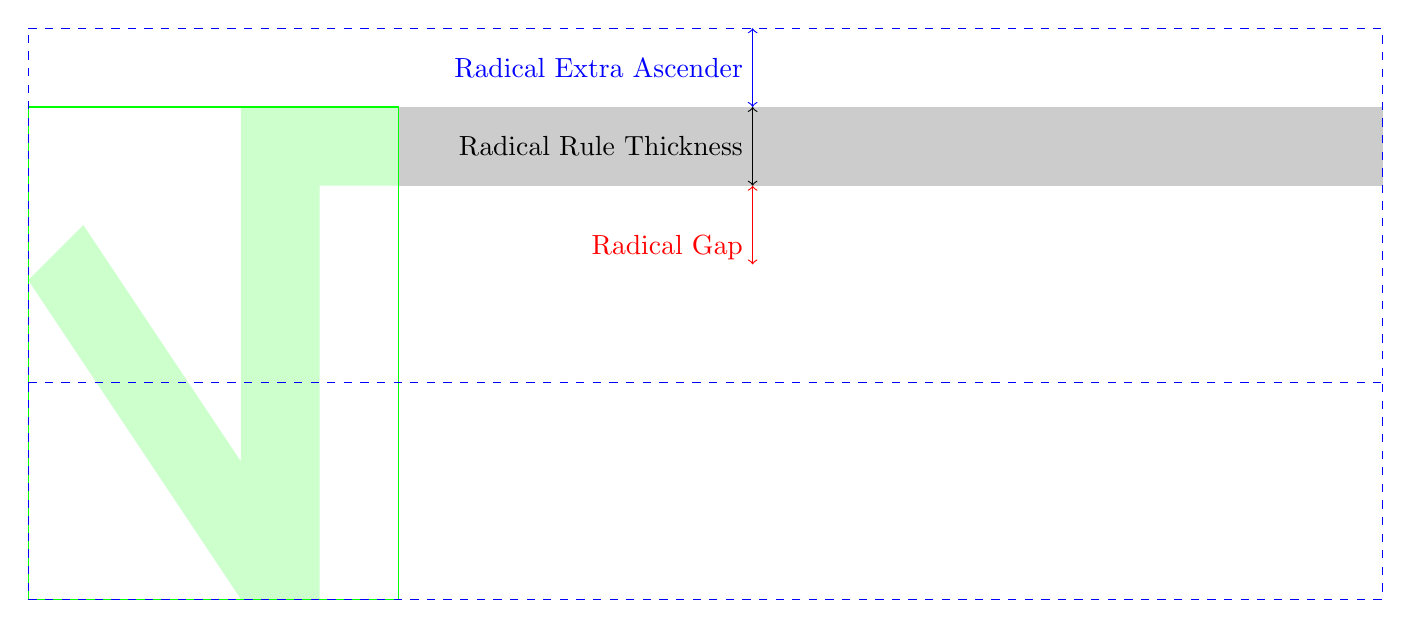
\begin{tikzpicture}[yscale=-1]

  \fill[black!20] (0,-2.5) -- (12.5,-2.5) -- (12.5,-1.5) -- (0,-1.5) -- cycle;

  \fill[green!20]
  (0,-2.5) -- (-2,-2.5) -- (-2,2) --
  (-4,-1) -- (-4.7,-.3) -- (-2.7,2.7) -- (-2,3.75) -- (-1,3.75) --
  (-1,-1.5) -- (0,-1.5) -- (0,-2.5);
  \draw[green] (-4.7,-2.5) -- (0,-2.5) -- (0,3.75) -- (-4.7,3.75) -- cycle;

  \MathMLBox{0}{1}{2.5}{1}{red}

  \draw[dashed,blue] (-4.7,-3.5) -- (12.5,-3.5) --
                     (12.5,3.75) -- (-4.7,3.75) -- cycle
                      (-4.7,1) -- (12.5,1);

  \draw[<->,blue] (4.5,-3.5) --
  (4.5,-3) node[left]{Radical Extra Ascender} -- (4.5,-2.5);

  \draw[<->,black] (4.5,-2.5) --
  (4.5,-2) node[left]{Radical Rule Thickness} -- (4.5,-1.5);

  \draw[<->,red] (4.5,-1.5) --
  (4.5,-1) node[below left]{Radical Gap} -- (4.5,-.5);
\end{tikzpicture}
\label{SquareRootBoxModel}
\end{figure}

The {\tt mroot} element is laid out as shown on figure \ref{RootBoxModel}.
We start by ignoring the root index and we layout the base and surd as
shown on figure \ref{SquareRootBoxModel} to obtain a box $B$.
The horizontal metrics of the {\tt mroot} element are obtained by putting
{\tt RadicalKernBeforeDegree}
before the root index, then placing the root index, then a kerning
of {\tt RadicalKernAfterDegree}
after the root index and finally placing $B$ (r. In general
the kerning before the root index is positive while the kerning after it is
negative,
which means that the root element will have some space before it and that the
root index will overlap the surd.
For the vertical metrics of the {\tt mroot} element, we first take the baseline
of $B$ as the baseline. Then if we graduate the ink height of $B$ with a linear
scale going from 0 (bottom) to 1 (top) then the baseline of the root index will
be vertically positioned at coordinate {\tt RadicalDegreeBottomRaisePercent}.
Finally, we take into consideration the box of the root index and $B$ to deduce
the metrics for the whole box of the {\tt mroot} element.

\begin{figure}
\centering
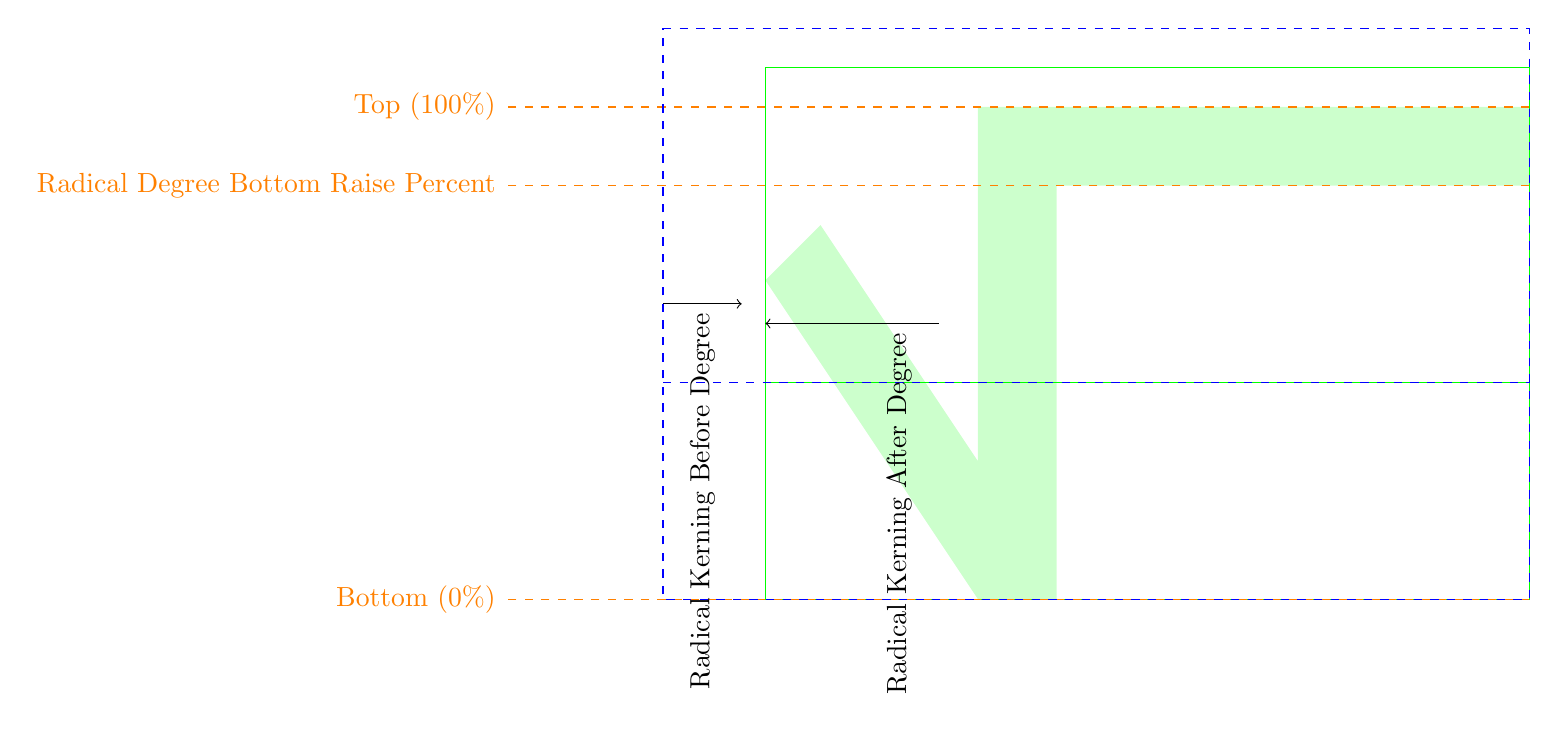
\begin{tikzpicture}[yscale=-1]
  \begin{scope}[shift={(6,0)}]
  \fill[green!20]
  (5,-2.5) -- (-2,-2.5) -- (-2,2) --
  (-4,-1) -- (-4.7,-.3) -- (-2.7,2.7) -- (-2,3.75) -- (-1,3.75) --
  (-1,-1.5) -- (5,-1.5) -- (5,-2.5);
  \draw[green] (-4.7,-3) -- (5,-3) -- (5,3.75) -- (-4.7,3.75) -- cycle
  (-4.7,1)--(5,1);
  \end{scope}

  \MathMLBox{1}{-1.5}{.5}{1}{red}

  \draw[dashed,orange](11,3.75)--(-2,3.75) node[left]{Bottom (0\%)};
  \draw[dashed,orange](11,-1.5)--(-2,-1.5) node[left]
       {Radical Degree Bottom Raise Percent};
  \draw[dashed,orange](11,-2.5)--(-2,-2.5) node[left]{Top (100\%)};

  \draw[dashed,blue] (0,-3.5) -- (11,-3.5) -- (11,3.75) -- (0,3.75) -- cycle
  (0,1)--(11,1);

  \draw[->,black] (0,0) -- (.5,0) node[left,rotate=90]
       {Radical Kerning Before Degree} -- (1,0);
  \draw[->,black] (3.5,.25) -- (3,.25) node[left,rotate=90]
       {Radical Kerning After Degree} -- (1.3,.25);
\end{tikzpicture}
\label{RootBoxModel}
\end{figure}

\subsubsection{Style Change {\tt <mstyle>}}

The MathML specification has a long description of {\tt mstyle} with several
ways to interpret the attributes, to handle inheritance and to deal with
additional exceptions. The most important points are \cite{MathML3}:
%
\begin{quote}
The {\tt mstyle} element is used to make style changes that affect the
rendering of its contents. [...]

The {\tt mstyle} element accepts a single argument, possibly being an inferred
{\tt mrow} of multiple children [...]

Loosely speaking, the effect of the {\tt mstyle} element is to change the
default value of an attribute for the elements it contains. Style changes work
in one of several ways, depending on the way in which default values are
specified for an attribute.
\end{quote}

For the layout algorithm described in this specification, the
{\tt mstyle} element must be treated the same as the {\tt mrow} element.
However, some attributes on the {\tt mstyle} element must be mapped to CSS
properties as indicated in section \ref{CSSProperties}.
All the other {\tt mstyle}
attributes not defined in this specification must be ignored.

\subsubsection{Error Message {\tt <merror>}}

The MathML specification describes {\tt merror} as follows \cite{MathML3}:
%
\begin{quote}
The {\tt merror} element displays its contents as an "error message". This
might be done, for example, by displaying the contents in red, flashing the
contents, or changing the background color. The contents can be any expression
or expression sequence.

{\tt merror} accepts a single argument possibly being an inferred {\tt mrow} of
multiple children. [...]
\end{quote}

For the layout algorithm described in this specification, the
{\tt merror} element must be treated the same as the {\tt mrow} element.
The user agent stylesheet (section \ref{UAStylesheet})
must set some CSS properties on the {\tt merror}
element in order to highlight the error. This can for example be achieved with
the rule:
%
\begin{lstlisting}
merror {
  outline: solid thin red;
  background-color: lightYellow;
}
\end{lstlisting}

\subsubsection{ Adjust Space Around Content {\tt <mpadded>}}\label{mpadded}

The MathML specification describes {\tt mpadded} as follows \cite{MathML3}:
%
\begin{quote}
An {\tt mpadded} element renders the same as its child content, but with the
size of the child's bounding box and the relative positioning point of its
content modified according to {\tt mpadded}'s attributes. [...]

The {\tt mpadded} element accepts a single argument which may be an inferred
{\tt mrow} of multiple children
\end{quote}

See \cite{MathML3} for how the metrics of {\tt mpadded} element are determined.
The height, depth and width of the content in \cite{MathML3} corresponds to
the logical box of the content. The content of the {\tt mpadded} element is
positioned from the origin of the {\tt mpadded} element as follows: We shif it
forward by a distance of {\tt lspace} and shift it upward by a distance of
{\tt voffset}. The logical metrics of the {\tt mpadded} element are given by the
height, depth and width of the {\tt mpadded} element described in
\cite{MathML3}. The ink metrics of the {\tt mpadded} element match their logical
metrics.

\begin{figure}
\centering
\begin{tikzpicture}[yscale=-1]
\end{tikzpicture}
\label{MpaddedBoxModel}
\end{figure}

...

\subsubsection{Making Sub-Expressions Invisible {\tt <mphantom>}}

The MathML specification describes {\tt mphantom} as follows \cite{MathML3}:
%
\begin{quote}
The {\tt mphantom} element renders invisibly, but with the same size and other
dimensions, including baseline position, that its contents would have if they
were rendered normally. [...]

The {\tt mphantom} element accepts a single argument possibly being an inferred
{\tt mrow} of multiple children [...]
\end{quote}

For the layout algorithm described in this specification, the
{\tt mphantom} element must be treated the same as the {\tt mrow} element.
The user agent stylesheet (section \ref{UAStylesheet})
must set some CSS properties on the {\tt mphantom}
element in order to hide its content. This can for example be achieved with
the rule:
%
\begin{lstlisting}
mphantom {
  visibility: hidden;
}
\end{lstlisting}

\subsubsection{Expression Inside Pair of Fences {\tt <mfenced>}}

The MathML specification has a long description of {\tt mfenced} with several
exceptions for the parsing of its attributes. It gives a strict equivalence
between {\tt mfenced} and constructions that rely exclusively on {\tt mo} and
{\tt mrow} elements Here is the main point \cite{MathML3}:
%
\begin{quote}
The {\tt mfenced} element provides a convenient form in which to express common
constructs involving fences (i.e. braces, brackets, and parentheses),
possibly including separators (such as comma) between the arguments.
[...]
\end{quote}

This specification does define any layout algorithm for the {\tt mfenced}
element. User agents may just treat them as equivalent to the {\tt mrow} element
or to an {\tt merror} element with a relevant error message indicating
unsupported markup.
Alternatively, {\tt mfenced} may be implemented using a shadow tree, anonymous
boxes, or any other methods that produce the same rendering as the equivalent
constructions with {\tt mo} and {\tt mrow} elements.

Authors are encouraged to use the equivalent constructions with {\tt mo} and
{\tt mrow} elements, instead of relying on the {\tt mfenced} element.

\subsubsection{Enclose Expression Inside Notation {\tt <menclose>}}

The MathML specification describes {\tt menclose} as follows \cite{MathML3}:
%
\begin{quote}
The {\tt menclose} element renders its content inside the enclosing notation
specified by its notation attribute. {\tt menclose} accepts a single argument
possibly being an inferred mrow of multiple children [...]
\end{quote}

...

\subsection{Script and Limit Schemata}

\subsubsection{Subscripts and Superscripts {\tt <msub>}, {\tt <msup>},
  {\tt <msubsup>}}

\subsubsection{Underscripts and Overscripts  {\tt <munder>}, {\tt <mover>},
  {\tt <munderover>}}

\subsubsection{Prescripts and Tensor Indices \tt <mmultiscripts>}

\subsection{Tabular Math}

...

\subsection{Elementary Math}

Elementary Math was introduced in version 3 of the MathML specification
\cite{MathML3}:

\begin{quote}
Mathematics used in the lower grades such as two-dimensional addition,
multiplication, and long division tends to be tabular in nature. However, the
specific notations used varies among countries much more than for higher level
math. Furthermore, elementary math often presents examples in some intermediate
state and MathML must be able to capture these intermediate or intentionally
missing partial forms. Indeed, these constructs represent memory aids or
procedural guides, as much as they represent ‘mathematics’.

The elements used for basic alignments in elementary math are:

{\tt mstack}: align rows of digits and operators
{\tt msgroup}: groups rows with similar alignment
{\tt msrow}: groups digits and operators into a row
{\tt msline}: draws lines between rows of the stack
{\tt mscarries}: annotates the following row with optional borrows/carries
and/or crossouts
{\tt mscarry}: a borrow/carry and/or crossout for a single digit
{\tt mlongdiv}: specifies a divisor and a quotient for long division, along
with a stack of the intermediate computations
{\tt mfenced}
[...]
\end{quote}

This specification does not define any layout algorithm for the {\tt mstack},
{\tt msgroup}, {\tt msrow}, {\tt msline}, {\tt mscarries}, {\tt mscarry} and
{\tt mlongdiv} elements.

\subsection{Enlivening Expressions}\label{maction}

The MathML specification describes {\tt maction} as follows \cite{MathML3}:
%
\begin{quote}
To provide a mechanism for binding actions to expressions, MathML provides the
maction element. This element accepts any number of sub-expressions as
arguments and the type of action that should happen is controlled by the
actiontype attribute. Only three actions are predefined by MathML, but the list
of possible actions is open.
\end{quote}
%
User agents must display at most one of the child of a {\tt maction} element.
User agents must determine the visible child as follows:
\begin{enumerate}
\item If {\tt actiontype} is {\tt toggle} and the {\tt selection} attribute
  (with default value 1) points to a valid child index
  between 1 and the number of children, then use the specified child.
\item If the {\tt actiontype} is {\tt statusline} or {\tt tooltip} then
  use the first child (if any).
\item Otherwise, the visible child is undetermined.
\end{enumerate}

For the layout algorithm described in this specification, the
{\tt maction} element must be treated the same as the {\tt mrow} element
containing its visible child. If it is undetermined,
the user agent may treat the {\tt maction} element as an
empty {\tt mrow} element or as an {\tt merror} element with some relevant error
message indicating invalid or unsupported markup.

User agents may additionally provide a complete implementation of the
{\tt toggle} actiontype updating the value of the {\tt selection} attribute
after the {\tt maction} element receives a {\tt click} event.
For {\tt statusline} and {\tt tooltip} attributes, they may also display the
second child in some way when the {\tt maction} element receives a {\tt hover}
event. This specification does not define how these DOM events are propagated
or how to change the default behavior.

Given the similarity with the {\tt semantics} element
(section \ref{semantics}), it is
suggested to share the implementation of {\tt semantics} and {\tt maction}.

\subsection{Semantics and Presentation}\label{semantics}

The MathML specification describes {\tt semantics} as follows \cite{MathML3}:
%
\begin{quote}
The {\tt semantics} element is the container element that associates
annotations with a MathML expression. The semantics element has as its first
child the expression to be annotated. Any MathML expression may appear as the
first child of the semantics element. Subsequent annotation and annotation-xml
children enclose the annotations. An annotation represented in XML is enclosed
in an {\tt annotation-xml} element. An annotation represented in character data
is enclosed in an {\tt annotation} element.
[...]
\end{quote}

User agents must display at most one of the child of a {\tt semantics} element.
For example, they may always display the first child (if any) or may use this
more advanced algorithm to determine a visible child:
\begin{enumerate}
\item If the {\tt semantics} element has a first child that is any of the
  MathML elements (other than {\tt annotation} and {\tt annotation-xml})
  whose rendering is described in this specification then use it as the visible
  child and stop.
\item Otherwise, check the children of the {\tt semantics} element in the DOM
  order to try and find the first child that is
  \begin{enumerate}
  \item Either an {\tt annotation} without any {\tt src} attribute.
  \item Or an {\tt annotation-xml} without any {\tt src} attribute and
    with an {\tt encoding} attribute that has value
    {\tt "application/mathml-presentation+xml"},
    {\tt "MathML-Presentation"},
    {\tt "image/svg+xml"},
    {\tt "SVG1.1"},
    {\tt "application/xhtml+xml"} or
    {\tt "text/html"}.
  \end{enumerate}
\item Otherwise, fallback to the first child (if any).
\item Otherwise, the {\tt semantics} element is empty and the visible child is
  undetermined.
\end{enumerate}

For the layout algorithm described in this specification, the
{\tt annotation-xml} element must be treated the same as the {\tt mrow} element,
the {\tt annotation} element must be treated the same as the {\tt mtext}
element. The {\tt semantics} element must be treated the same as an
{\tt mrow} element containing only its visible child. If it is undetermined,
the user agent may treat the {\tt semantics} element as an
empty {\tt mrow} element or as an {\tt merror} element with some error message
indicating invalid markup.

Given the similarity with the {\tt maction} element
(section \ref{maction}), it is
suggested to share the implementation of {\tt semantics} and {\tt maction}.
